\documentclass[a4paper]{article}
\usepackage[utf8]{inputenc}
\usepackage{indentfirst}
\usepackage{biblatex}
\usepackage[table]{xcolor}
\usepackage{graphicx}
\usepackage[left=2.5cm,top=3cm,right=2.5cm,bottom=3cm,bindingoffset=0.5cm]{geometry}

\definecolor{light-gray}{gray}{0.9}

% \setlength{\textheight}{690pt}
% \setlength{\topmargin}{-0.3in}
% \setlength{\headsep}{0pt}
% \setlength{\oddsidemargin}{-6mm}
% \setlength{\textwidth}{7in}

\title{CS 253: Final Project Report}
\author{Ildar Absalyamov \and Longxiang Chen \and Ali Mohammadkhan}

\addbibresource{references.bib}

\begin{document}

\maketitle

\section{Introduction}

The Internet and computer networks were initially designed with the idea that equipment, carrying individual packets, is faulty and unreliable.
This premise heavily influenced on the implementation of OSI reference model.
Transport layer protocols of this model (TCP as the most popular) provide users with the abstraction of reliable data packets transfer channel, however the implementation of this interface is build on top of noisy, volatile and inherently unreliable network \cite{deutsch1992eight}.
In the network packets could be sporadically dropped, delayed, duplicated and reordered.

To maintain this abstraction TCP implements statefull handshake algorithm to ensure that transfered data was reliably received on the destination node, but it comes with the cost of increased transmission latency.
Basically, that means that any operation on the client is blocked, until it will receive an acknowledgment, that the transmission was delivered successfully. 
In particularly noisy networks there is no any guarantee that this acknowledgment would be received at all, so theoretically client could wait forever.
In practice clients usually have some reasonable timeouts, which are used to determine whether the transmission has succeed or not.

In the following work we will be focused on particular type of network failure, called partition.
Network partition is failure in which a topology is divided into two (or more) parts, which are separated from each other.
Nodes inside each partition are able to communicate with each other, but they cannot reach servers in the other partitions.

The probability of network partitioning depends on the topology of the network, which in the worst case could be connected through one (or small group) of nodes.
Crash of these nodes would lead to violation of network connectivity.

Partitioning is a big issue for Internet traffic, where there is no way to determine the whole topology of the network.
For a long time it was considered that the partitions inside the data centers occur extremely rarely, however data \cite{aphyrNetworkStatics,dean2009designs} collected from the companies like Google, Amazon, etc, which have tens of data centers scattered around the globe, shows that even with high intra-datacenter redundancy partitions still could emerge.
Or course the time, during with network is partitioned, is minuscule in comparison with the uptime of servers, but for distributed applications working under the high load (which are usually deployed in these data centers) even slight failure could cause a lot of troubles.
Loss of communication, happened due to network failure, could cause local copies of the data to diverge.
If the application is not aware of partitioning it could end up with incorrect state, after the network connectivity is restored.
What is even worse, is that the application never be sure, whether a request, failed due to partitioning error, will never be processed . 
The failure could be caused by network timeout, which, in the case of a slow network, does not imply that the original request will not arrive later.

In distributed setup partitioning is the inherently connected with other properties of distributed systems like availability and consistency \cite{brewer2000towards}.
Surprisingly, limited number of experimental research has been done on distributed systems, when their networks have faced network partition challenges. 
The goal of current project is to make a case study for different distributed storage systems, measuring how these systems would perform under the assumption of network partition in the cluster.

\section{Related Work}

Although, it might seem that research in a area of distributed systems was actively done only during past decade, this fields captured an attention of academia long time before.

The seminal paper by Davidson et al. \cite{Davidson:1985:CPN:5505.5508} already was describing the properties of distributed systems with replicated data, working in partitioned networks.
This work was the first, discussing the tradeof between consistency and availability in a case of lack of network connectivity.
However it was assuming that modifications are executed in transactional context, thereby allowing only strong linearizable consistency guarantees.
This approach was proved to be non-scalable in real distributed setup.

Later work by Fox et al. \cite{fox1997cluster} discussed possible ways to relax consistency guarantees in order to maintain reasonable performance for application with data intensive workload. 
It was first to propose BASE (basically available, soft state, eventual consistency) semantics instead for known ACID (atomicity, consistency, isolation, durability) transaction, which were implemented in database system for decades.

The following work by Brewer \cite{brewer2000towards} synthesized all existing research in a form of famous CAP-theorem, which was alter formally proved by Gilbert et al. \cite{gilbert2002brewer}.
CAP-theorem establishes inherent relationship between availability and consistency properties of distributed system, working in partitioned networks, and formulates theoretical bound (in terms of maintained properties) for any of such systems.

All these works led to rise and proliferation of the whole new type of database system, called NoSQL storages \cite{strauch2011nosql}.
This name consolidates a set of diverse distributed storage systems. 
Implementation and basic principles of these systems vary considerably, from dynamically scalable systems with identical nodes and ring-like structure \cite{decandia2007dynamo} to systems with structured data model and implicit distinction between masters and slaves in the cluster \cite{chang2008bigtable}.

Experimental evaluation of these heterogeneous systems, emerging every so often, quickly became a big issue.
Albeit CAP-theorem bounds the functionality of these systems it given only a theoretical upper bound.
The real implementation could claim to maintain certain characteristics, like consistency and availability.
But in reality in border situations, like slow network, dropping part of packets or temporary network partition, it could demonstrate completely different behavior, violating proclaimed guarantees.

Only recently these emerged a work \cite{jepsen}, which tried to create an evaluation framework for measuring systems behavior under assumption that network is partitioned.
Some popular distributed data storages like Cassandra \cite{lakshman2010cassandra}, MongoDB \cite{mongo}, Redis \cite{redis}, Riak \cite{riak}, etc were used in this study.
The following work presents a case study, that tries to follow the same approach, for performance evaluation of various distributed databases.

\section{Selected storage systems}
\label{sec:candidates}

\subsection{Hazelcast}
Hazelcast is distributed highly scalable in-memory grid, providing distributed access to the typical data structures (Maps, Queues, Lists, Sets) partitioned across the cluster. 
Hazelcast is peer-to-peer system without any single point of failure problem.

It supports multi-datacenter configuration via WANReplication feature with active-active and active-passive replication configurations.

Hazelcast also allows user to pick how many replicas maintain across the cluster and what conflict resolution strategy to use, in the case of conflicting entries.  

\subsection{Couchbase}

Couchbase is a distributed scalable document-oriented database, which runs on shared-nothing clusters.
In terms of CAP theorem Couchbase is a typical CP system which means that it sacrifices availability for keeping stored data consistent.
However, it has a failover option that changes its behavior dramatically. 
In order to explain failover feature in details, at first we briefly talk about Couchbase architecture and VBucket concept, then we describe the failover option and finally we explain what is rebalancing in Couchbase and why it is necessary.


\subsubsection{Couchbase structure}
As it was mentioned earlier, Couchbase is a document-oriented database, so the entities stored or retrieved from the database are documents. 
Each document is indicated by a key.
Couchbase uses the document's key to assign it to particular VBucket. 
VBucket (or virtual bucket) is an abstract concept, which does not really exist on servers, but Couchbase uses this concept to distribute data among different servers. 
To assign VBuckets to servers, Couchbase uses a special table shown in Figure \ref{fig:vbucket}.

\begin{figure}[h!]
\centering
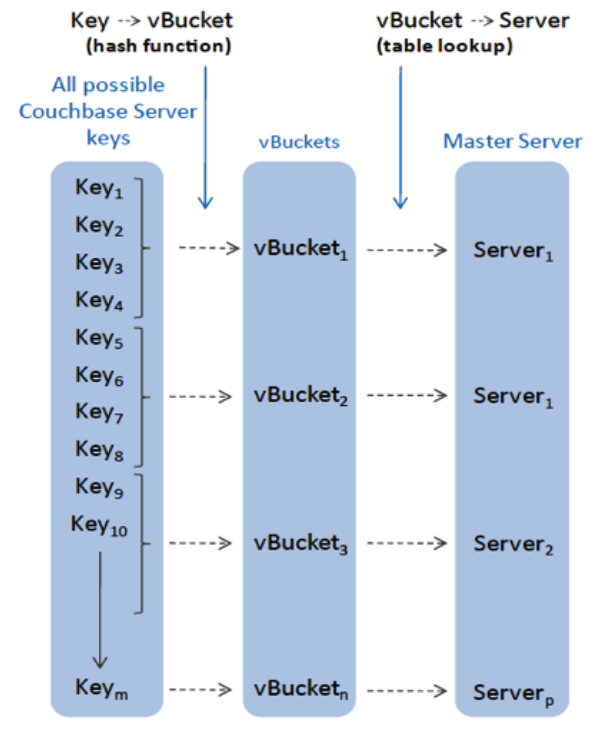
\includegraphics[ height=300pt]{vbucket}
\caption{Document assignment to servers procedure in Couchbase \cite{memcachedchallenges}}
\label{fig:vbucket}
\end{figure}	

\subsubsection{Couchbase failover feature}
Failover is the process of expulsion of server from the cluster. 
If failover procedure is activated on the node, this server loses it membership in a cluster and it cannot rejoin to the cluster even after healing back. 
The failover can be done manually or automatically. 
The automatic failover is de-activated by default, but you can easily activate it by using the web console of Couchbase. 
The automatic failover procedure will be started after a period of time that a server not responding to others.
The minimum and default value for this period is 30 seconds. 

\subsubsection{Couchbase rebalancing feature}
After expelling a server from the cluster using failover procedure, we need to rebalance the cluster. 
The rebalancing procedure is necessary because the number of active servers in the cluster has changed and some of VBucket assignment are not valid anymore.
When the rebalancing procedure is finished, we will have new VBucket assignment and some documents may be transferred to another server.


\subsection{Voldemort}

Voldemort is a distributed key-value storage system, providing tunable consistency (strict quorum or eventual consistency). It is used in LinkedIn for certain 
high-scalability storage problems where simple functional partitioning is not sufficient. 

Voldemort combines in memory caching with the storage system so that a separate caching tier is not required. Unlike MySQL replication, the reads and writes scale horizontally. It also allows cluster expansion without rebalancing all data.

Voldemort provides simple API for data replication and placement, which makes it easy to accommondate a wide range of application specific strategies.


\section{Implementation}

These tests are similar for all three candidate storage systems in essence, but due to the specific characteristics of each system the details could differ. 
For instance, some storage systems have peer-to-peer nature while the others have master-slave architecture, each of these categories needs different test scenarios to be able to carry out comprehensive tests.

Our setup consists of five virtual machines, with Ubuntu Linux installed on all of them along with the considered data storage system. 
These five nodes are connected into a single virtual network, which is located behind a NAT separating it from the host system.
To be able to communicate with the individual nodes of the storage system, we implemented a small client application which was running on a host system, whose requests were routed through the NAT to designated cluster nodes. 
Overall configuration in shown on Figure \ref{fig:cluster}. 

In order to simulate the network partition in this cluster and disconnect nodes N1 and N2 from nodes N3,N4,N5 we configuring iptables firewall on each cluster node to drop packets, received from the partitioned part of the cluster.
Note that the host system is always connected to the cluster nodes, so the partition exists only form the node's point of view.

\begin{figure}[h!]
	\centering
	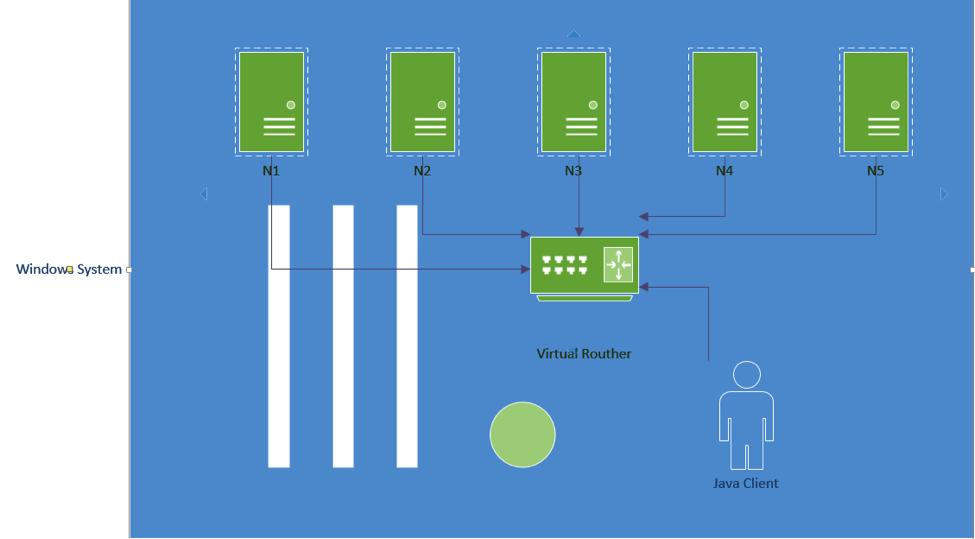
\includegraphics[width=\textwidth]{cluster}
	\caption{Virtual cluster}
	\label{fig:cluster}
\end{figure}

\section{Evaluation}

\subsection{Hazelcast}

For the set of experiments cluster of hazelcast version 3.1 was deployed on the worker nodes. 
We have tested two types of configuration: local cluster and several clusters with WAN replication, each of which was declaring a single distributed map, which was written from the individual worker node.

Tests for the local cluster reveled that out of 2000 writes almost 10\% are lost (result depends on the length of the period, during with the partition was present).
Results show that every record, written on the smaller partition (nodes N1 and N2) is lost, even after partition disappears, which clearly shows the issue with distributed consensus algorithm, used in Hazelcast.
Also it could be noted that when the partition is resolved latency of writes, going to nodes N1 and N2 temporarily increases, which could be explained by the fact that the tuples on these nodes should migrated, when they are rejoining the cluster.

On the other hand configuration, which used WAN replication perfectly survived the network partition, returning all 2000 successfully written tuples.

{\bf To be completed...}

\subsection{Couchbase}

In our experiments we have used Couchbase 2.1.1, which is the latest available Community edition version. 
Since Couchbase is a peer-to-peer system, there is no need to manually set up master node. 
Servers obtain their configuration from each other in a peer-to-peer way.

To start testing and checking the configuration we wrote and later read 1000 documents to Couchbase system and all of them were successful. 
The data is distributed approximately evenly among different servers (each server stores about 200 documents).
Replication factor is equal to 1, means that a replica of each document is stored somewhere on another server.
When the Couchbase system is under stress (for example when virtual machines do not have access to enough RAM), we observe that sometimes the client code throw exceptions in writing data.
However after checking the written data, that data exist on Couchbase, so we conclude that exception always is not a sign of unsuccessful write.  

When one of the servers is turned off, about 20\% of our writes ended up being lost.
In other words, just 803 documents were written into Couchbase successfully, and the client was attempting to write other documents to server N5 in a loop.
The loop was infinitely executing as long as the node N5 was down.
After writing documents to servers, if the N5 remains being unconnected and is expelled from the cluster using failover procedure, we were able to successfully read all the written documents.
The successful reading are result of replication in Couchbase system.

For the network partition tests with deactivated failover, all writes and reads were successful.  
However, the number of replicas were reduced in comparison to prior test, so it lead us to design the next test. 
In this test we also measured the number of reads and writes per second that are acknowledged in normal and network partition situations.
The result was approximately the same in both conditions.

In this test, after writing the 1000 documents in partitioned mode, we turned off the N5 server and we started failover process manually.
This time we just were able to read 850 data documents out of 1000 written documents in first place. 
It shows that the replication policy of Couchbase was not successful in presence of network partition.

In the next test, we introduced network partition while we were writing documents to Couchbase database and we started failover procedure prior to finishing of the writing process. 
About 24\% of writes were not successful, although this amount depends on the time, when the partition was introduced and failover procedure was started, and may vary between different tests.
After document writes were finished, just about 15\% of these documents could be read from one partition and 66\% could be read from another partition.
You may noticed the fact, that the total number of documents that have been read, is more that the number of written documents.
As we mentioned before, the reason is that some unsuccessful written are not really unsuccessful and they are counted as unsuccessful because acknowledgment for these operations was was received, due to thrown exceptions. 
We had stored some other documents before writing this series of documents, 70\% and 90\% of them could be read from these two different partitions.
Again the total is more than 100\% , but this time the reason is that some documents are retrieved from available replications. 
Then we fixed the partition and rebalanced the cluster again, 90\% of old documents and 15\% of new documents could be read from the joined cluster.
It means that we lost the document stored on one of our partitions.

\subsection{Voldemort}

In the beginning, we proposed to use RethinkDB as a third storage system, that we would like to evaluate. But this database is not well documented because it is a new system that few people use it. So it would be hard to configure RethinkDB to support multi-datacenter replca set.

Our backup option was to use Voldemort distributed key-value storage and configure it for replica set support. Different from the previous two (CP) database systems, Voldemort is a Availability-Partition Tolerant(AP) system. 

We set the quorum factor as following:

\begin{table}[hb]
  \centering
  \begin{tabular}{|c|c|c|}
    \hline
    replication (N) & 5 & Final number of replications in the system. \\
    \hline
    required-write (W) & 3 & Least number of writes w/o throwing an exception. \\
    \hline
    required-read (R) & 3 & Least number of reads w/o throwing an exception. \\
    \hline
  \end{tabular}
\end{table}

At the first stage, we opened only two nodes (N1-N2), then all write operations received exception, indicating that the write was failed. 
Because the replication could not be executed successfully (since W = 3), the database system throws an exception back to the client. 
When we woke up the third node (N3) to meet the least number of nodes for required-writes and required-reads, the client was able to read the objects we wrote before, even though this writes were unsuccessful, and should not be a part of result set. 
Voldemort implements ``Hinted Handoff'' technique, used to maintain eventual consistency semantics. 
During writes, if the destination nodes are down, Voldemort stores a ``hint'' of the updated value on one of the alive node. 
As soon as the down nodes are alive again, the ``hints'' will be pushed to them. 
Based on this technique, Voldemort can keep the data consistent even when the required-write quorum cannot meet.

The next step was to test the five nodes with network partitions as it was mentioned before. 

{\bf Steps:}
\begin{enumerate}
  \item Start running Voldemort in 5 VMs, 5 clinets keep writing distinguished data to their correspoding nodes.
  \item Use iptables to create a network partition between N1/N2 and N3/N4/N5 for a while(20 sec.), the clients keep writing data.
  \item Remove the blocking IPs from iptables' list (network recovered), before all writes are done.
  \item After all writes in one node is done, each client check the data in its node independently.
\end{enumerate}

{\bf Results:}
\begin{enumerate}
  \item Nothing happens, Voldemore does not return anything if the write/read is successfully.
  \item After network partition starts, clients of N1 and N2 receive exceptions because the required-write (W = 3) cannot meet. N3/N4/N5 keep the same as the above. 
  \item All nodes go back to result 1 as the network partition is removed.
  \item Finaly, each node finishes exchanging their data for replicas. Then all nodes have a final replications (N = 5) of all data objects.
\end{enumerate}

In the final set of all data, there some objects were missing. 
Based on the first stage, we found that Voldemort could handle writes when the node, we are writing to, is down. 
Performance of hinted handoff may depend on the number of objects, which should be temporarily stored. 
During the network partition period (20 seconds), if the number of writes with exceptions was not large (1 write/second, 20 writes in total), Voldemort was able to handle all of them after network partition is removed. 
However, if the number of failed writes is large (10 writes/second, 200 in total), Voldemort would drop some of the objects, so some objects will end up missing. 
In both cases, the number of exceptions the clients received is larger than the number of missing objects. 
The objects to write are failed to meet the required-write (W = 5), so Voldemort throws an exception. 
However, hinted handoff allows the database to store some (may not all) of the failed objects, and write them back to the recovered nodes later. 
This may result in a higher number of exceptions than missing objects in the end.

\subsection{Conclusions}

{\bf To be completed...}

In Couchbase, when failover feature is off, it performs very well under network partition and it is a real reliable CP system.
However the problem is that the availability has been sacrificed extremely, for instance you cannot read or even write documents assigned to a VBucket on a down server until it comes back.
Therefore you have no way but activating the failover feature. 
When this feature is activated, the availability problem is solved but it is not a consistent database anymore and lots of documents, including the ones which were successfully written, may end up being lost. 

Another downside of Couchbase under network partition is that, its replication policy is not fully functional anymore.
It means that you may lose some part of your documents even by failure just in a single server.

For the Hazelcast , it does not guarantee strong consistency. In different test cases or configurations, the performance of it
vary significantly.
For the AP systems (Voldemort), the availability is pretty good, almost all the writes are succesful eventually, with a failure rate around 5/2000 = 0.25\%.
Exceptions does not indicate 100\% write failure, rather it does say that we do not know where the objects are.

To sum up, designers and developers of distributed storage systems have not considered the devastating effects of network partition as much as needed.
Maybe they have trusted too much to network infrastructure which is not a wise decision because network is unreliable in its nature.
We think that distributed storage community deeply needs to reconsider its procedure against network partition.
If not, storage systems will not be enough consistent and reliable for enterprise users.


\section{Future Work}
In this paper we investigated the network partition problem in three different distributed storage systems, but we did not implement any solution to mitigate or solve the problem of network partition in these systems. 
A partition aware script along with these systems can reduce the impact of this problem before being addressed by developer of these systems.
In addition, various distributed storage systems exist and lots of them are not robust in network partition situations.
Just few of these storage systems are investigated under network partition condition.
It seems useful to have these systems tested and inform the user of these systems about probable shortages of these systems under network partition.


\section*{Contribution}

\begin{table}[h]
	\centering
	\begin{tabular}{|c|c|}
		\hline
		\rowcolor{light-gray} \textbf{Contributor} & \textbf{Experiments} \\ \hline
		Ildar & Hazelcast  \\ \hline
		Lonxiang & Voldemort  \\ \hline
		Ali & Couchbase  \\ \hline
	\end{tabular}
\end{table}

\printbibliography

\end{document}